
%***********************************************************************

% This is a template to be used for the preparation of
% papers submitted to the 33rd International Workshop on
% Statistical Modelling, to be held in Groningen, Netherlands,
% July 15-20, 2018.

% Please follow the following general guidelines:
%
% (1) Do not specify any definitions, commands or style parameters.
%     Upon submission, your file will be checked for presence of
%     \newcommand or \def statements and if found, error message will be reported
%     by the submission form.
%
% (2) Follow the template below very tightly.
%
% (3) Include .pdf figures using the \includegraphics
%      command, an example of which are given below.
%
% (4) Use file names which begin with the surname of the first author.
%
% (5) When creating labels for cross-references, please start always
%     by surname of the first author, e.g., \label{smith:likelihood}
%
% (6) The template below contains some example materials
%      to guide you through the preparation of your paper.  However,
%      remove all the redundant material from your final document
%      before submitting.

% The guidelines above are needed in order to be able to combine all
% the papers into a single proceedings book of acceptable quality.
% Please follow the guidelines as strictly as possible. Deviations may
% result in papers being either refused by the registration form
% or sent back to the authors with the request to change
% their documents according to the guidelines.

% Special characters:
% Please do not use special characters (e.g., accents).
% Use TeX composition instead, such as \~n, \'a, \`e, \v{s}, \r{u} etc.

% Changes as of IWSM 2013:
%  * \usepackage{booktabs} added which allows \toprule et al. in the tabular environment
%    (\hline\hline is not longer used)
%  * '^\T' added in iwsm.sty to denote transposed vectors and matrices within math (see example below)
%  * \usepackage{amsmath, amssymb} introduced since IWSM 2012 is allowed (allowing usage of boldsymbols
%    and other handy constructions (align, pmatrix etc.) within math)
%  * \usepackage{psfrag} introduced since IWSM 2012 is NOT allowed
%
%

%***********************************************************************
% PLEASE LEAVE THIS PART UNCHANGED
%***********************************************************************

\documentclass[twoside]{report}
\usepackage{iwsm}
\usepackage{graphicx}
\usepackage{amsmath, amssymb}
\usepackage{booktabs}

% Please do not specify any new definitions, any new commands,
% and do not specify any style parameters.
% The preamble of the document should be left unchanged.

% proofreading
\usepackage[textsize=scriptsize, backgroundcolor=lightgray, draft]{todonotes}
% ab todo note definition
\newcounter{todocounter}
\newcommand{\abtodo}[1]{
  \stepcounter{todocounter}\todo[color=black!30]{
    \textbf{AB[\thetodocounter]: }#1
  }
}

\begin{document}

%***********************************************************************
% PLEASE INSERT YOUR CONTENT FROM HERE
%***********************************************************************

% Title and running title to be used as left header:
\title{KOALA: Estimating coalition probabilities in multi-party electoral systems}
\titlerunning{Short title used as left header}

% Authors and running list of authors to be used as right header:
\author{Alexander Bauer\inst{1}, Andreas Bender\inst{1}, Andr\'e Klima\inst{1}, Helmut K\"{u}chenhoff\inst{1}}
\authorrunning{Bauer et al.}    %% use \authorrunning{Surname 1} if only 1 author
                                    %% use \authorrunning{Surname 1 and Surname2} if two authors
                                    %% use \authorrunning{Surname 1 et al.} if more than two authors

% Institutes of all authors
% Include city and country of each institute, do not include the full address.
\institute{Statistical Consulting Unit, StaBLab, Department of Statistics, Ludwig-Maximilians-Universit\"{a}t, Munich, Germany}

% E-mail of presenting author for correspondence
\email{Alexander.Bauer@stat.uni-muenchen.de}

% Brief abstract of the paper:
\abstract{
Common election poll reporting is often misleading as sample uncertainty is either not covered at all or only insufficiently. For a more comprehensive coverage, we propose shifting the focus towards reporting survey-based probabilities for specific election outcomes. We present such an approach for multi-party electoral systems, focusing on probabilities of coalition majorities. A Monte Carlo based Bayesian Multinomial-Dirichlet model is used for estimation. The method utilizes opinion polls conducted by established polling agencies and is accompanied by a pooling approach to summarize multiple current surveys, accounting for dependencies between institutes.
%Potential biases of specific pollsters are not taken into account.
Sample uncertainty-based probabilities are estimated, assuming the election was held today. An implementation of the method in \texttt{R} is freely available.
}

% Keywords (at most 5):
\keywords{Election analysis; Opinion polls; Election reporting; Multinomial-Dirichlet; Pooling.}

% Produce the title:
\maketitle
\abtodo{Es is entweder Ludwig-Maximilians-Universit\"{a}t M\"{u}nchen oder LMU Munich}

%***********************************************************************

% Sections and subsections (do not use lower levels):

\section{Introduction and data}
\abtodo{Mit dem Satz stimmt iwas nicht: Election polls as surveys ...}
Election polls as surveys conducted by different polling agencies try to represent the public opinion based on a finite sample. Current reporting on such surveys is most often limited to the observed shares, while sample uncertainty and the multinomial structure of the data is usually ignored. Often e.g., a coalition is stated to ``lose'' its majority just because the joint poll share drops under 50\% (cf. ``Umfrage zur Bundestagswahl'', 2017).
In our opinion, the focus in survey reporting in multi-party electoral systems should be shifted towards the most relevant question, i.e. \textit{how probable} an event, e.g., a majority for a specific coalition is.
\abtodo{Begriff coalition wurde noch nicht eingeführt. Ggf. ganz am Anfang sowas wie: In multi-party electoral systems, one party usually doesn't obtain enough votes
for a majority. In these situation, multiple parties form a so-called coalition to obtain the necessary majority shares.}
We present our KOALA (Coalition Analysis) approach to estimate such probabilities
to bring more value to opinion poll-based reporting.
Prior to the German federal elections 2013 and 2017, results based on (an earlier iteration of) our approach already entered general media reporting (cf. ``Serie:~Wahlistik'', 2013, or Gelitz, 2017).

As database, we use opinion polls conducted by established polling agencies,
quantifying the electoral behavior \textit{if an election was held today}.
Our approach is to be differentiated from prediction-aimed methods (cf. Graefe, 2017 or Norpoth \& Gschwend, 2010). We focus on the question of quantifying current majority situations, not taking into consideration potential shifts until election
day.

A Bayesian Multinomial-Dirichlet model with Monte Carlo simulations is used for estimation. Also, a pooling approach is presented to summarize the results of multiple current opinion polls to reduce sample uncertainty.

All methods were implemented in \texttt{R} and are available in the open-source
package \texttt{coalitions} on GitHub (Bender \& Bauer, 2018). Also, an
interactive \texttt{shiny}-based (Chang et al., 2017) website \texttt{koala.stat.uni-\allowbreak muenchen.\allowbreak de}
visualizes estimated coalition probabilities and is used to communicate the
results to the general public.



\section{Calculation of probabilities}
As an example, we look at the last opinion poll conducted before the German federal election 2013 (Forsa, 2013), where special interest was on whether CDU/CSU-FDP (also ``Union-FDP'') would obtain enough votes to form the governing coalition:
\begin{table}[!ht]\centering
\caption{\label{bauer:tab_fdp} Observed voter shares in the Forsa opinion poll published September 20th, 2013 with $n=1995$ respondents}
\medskip
\begin{tabular}{cccccccc}
\toprule[0.09 em]
Union & SPD & Greens & FDP & The Left & Pirates & AfD & Others \\
\midrule
40\% & 26\% & 10\% & 5\% & 9\% & 2\% & 4\% & 4\% \\
\bottomrule[0.09 em]
\end{tabular}
\end{table}
\vspace{2ex}

The German election system mandates a 5\% votes share for each party to enter the parliament, thus
votes for parties below this threshold are redistributed (proportionaly) to parties
above the 5\% threshold.
\abtodo{Ich würde hier noch klarer rausarbeiten, dass das wichtig ist, weil deutlich
weniger als 50\% notwendig sind, um Mehrheit zu bekommen. Dann ist auch
weiter unten klarer warum Betrachtung der AfD hier notwendig ist.}
Here, Union-FDP would get exactly 50\% of parliament seats. Uncertainty-ignoring reporting would in this case conclude that the coalition slightly fails to achieve a majority. However, it is clear that this is only true with a specific probabilitiy and particularly depends on whether FDP and/or AfD pass the 5\% hurdle.


To estimate \emph{probabilities} for specific coalitions, we choose a Multinomial-Dirichlet model with an uninformative prior for the true party shares
$\theta_j$ (Gelman et al., 2013):
$$
\begin{aligned}
\boldmath{\theta} &= (\theta_1,\ldots,\theta_k)^\T \sim Dirichlet(\alpha_1,\ldots,\alpha_k), \\
\text{with} &\ \ \ \ \ \ \ \ \ \ \ \ \ \ \ \alpha_1 = \ldots = \alpha_k = \frac{1}{2}
\end{aligned}
$$
Given one (pooled) survey, the posterior also results in a Dirichlet distribution
with parameters $\alpha_j = x_j + \frac{1}{2}$ for each party $j$ and its observed
vote counts $x_j$.

Using Monte Carlo simulations of election outcomes, one can easily obtain
probabilities of specific events, by calculating the relative frequency of their
occurence in the simulations. As vote shares are usually rounded before publication,
we adjust the available data by adding random noise to $x_j$ before
calculating the Bayesian posterior.
\abtodo{Nach Möglickeit sollte man schon die Details zum ``random noise'' einfügen,
sonst ist es nicht klar was das sein soll.}
%we add uniformly distributed random noise $r_\gamma \sim U[-\gamma,\gamma]$ to the shares (e.g., $\gamma = 0.5\%$) and rescale the sum to $100\%$.

For visualizing
\abtodo{Du benutzt die *ing Grammatik zu oft. Glaube auch es ist kein richtiges
Englisch ``For *ing''. Einfach: To visualize...}
the development of such probabilities together with the underlying uncertainty for a specific coalition we recommend using a density plot
\abtodo{Ridgeline Plots ist die offizielle bezeichnung, siehe citation(ggridges)}
for its simulated seat distribution (Fig.~\ref{bauer:dens}). Looking at the probabilities based on the last opinion poll before the German election 2013, the posterior distribution ends up to be a bimodal distribution, based on the distinction whether FDP and/or AfD pass the 5\% hurdle. The resulting probability for a Union-FDP majority is \textcolor{red}{XXX\%}, based on \textcolor{red}{XXXX} simulations.


\begin{figure}[!ht]\centering
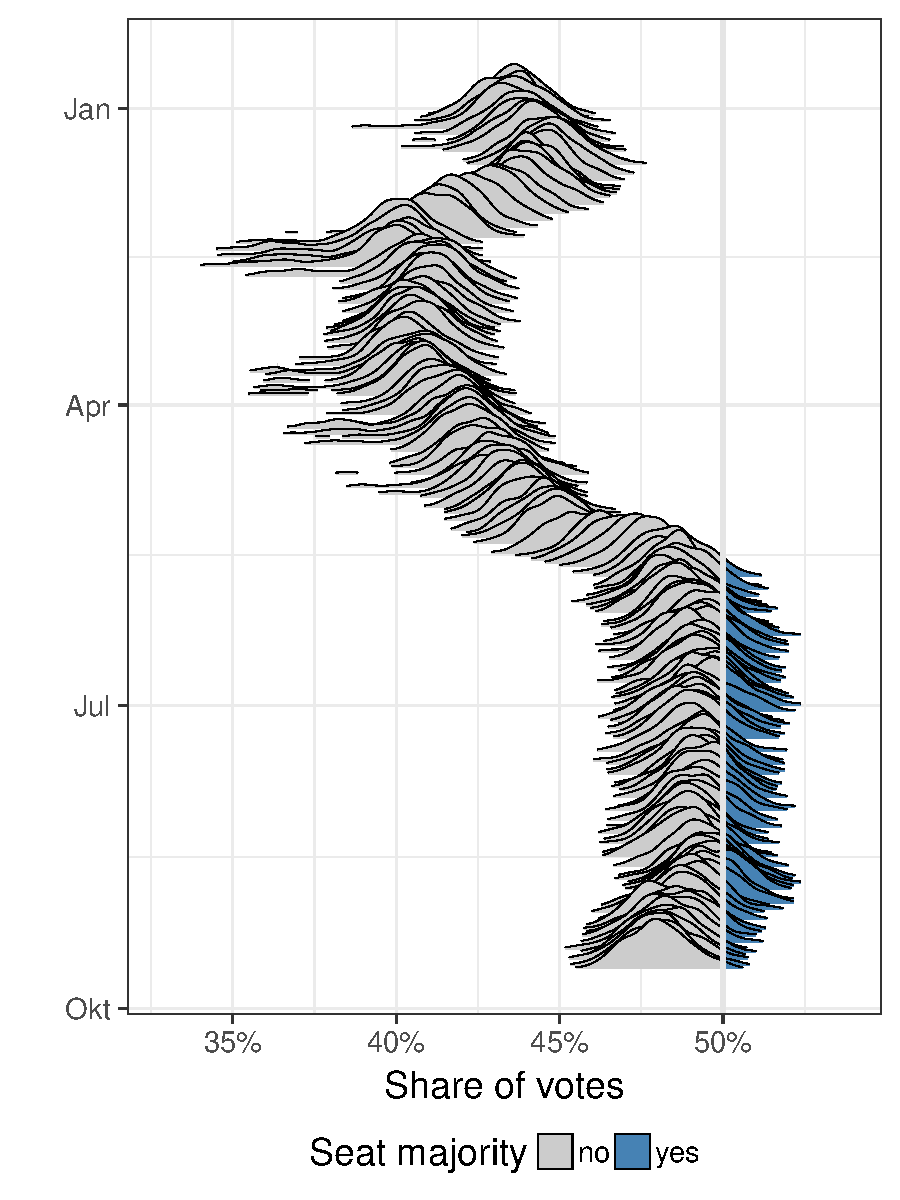
\includegraphics[width=0.4\textwidth]{figures/bauer_seatDist_time.pdf}
\caption{\label{bauer:dens} Development of simulated parliament seat share densities for the coalition Union|FDP before the German federal election in September 2013 based on Forsa. The density area colored blue marks the part of the density encoding for seat majorities. \textcolor{red}{Bimodale, letzte Umfrage muss noch in die Grafik. Und die Grafik muss auf Forsa basieren, nicht auf gepoolt! Und xlab = share of parliament seats}}
\end{figure}
\abtodo{Würde auch lines der density plots heller machen/transparent, falls die
Grafik die aktuelle größe beibehält. Um Platz zu sparen, kann man hier mehrere
Grafiken selber Größe nebeneinander einfügen.}



\section{Pooling approach}
In the presence of multiple published opinion polls, pooling is used to summarize the observed results in order to reduce sample uncertainty. To assure a reliable pooling regarding the current public opinion, we only use polls published within the past 14 days and only use the most recent survey published by each polling agency.

% Looking at a single poll $i$, the observed number of votes $X_j$ for each of $k$ parties follow a multinomial distribution with sample size $n_i$ and underlying, unknown party shares $\theta_j$ in the population:
% $$
% X_1,\ldots, X_k \sim Multinomial(n_i,\theta_1,\ldots,\theta_k).
% $$
Based on the multinomial distribution of the vote counts $X_{ij}$ of party $j$ in poll $i$ with underlying true party share $\theta_j$, pooling over multiple polls representing independent random samples would lead to a multinomial distribution for the
summed number of votes $\sum_i X_{ij}$.
% $$
% \sum\limits_i X_{i1},\ldots, \sum\limits_i X_{ik} \sim Multinomial(\sum\limits_i n_i,\theta_1,\ldots,\theta_k).
% $$

Further investigations, however, show that polls from different
polling agencies are correlated and the independency assumption
does not hold. Therefore, we adjust the resulting
multinomial distribution by using an \textit{effective sample size} (Hanley et al. ,2003). The necessary party-specific correlations were estimated from
20 surveys of the polling agencies, Emnid and Forsa, based on equation
$$
Cov(X_{Aj}, X_{Bj}) = \frac{1}{2} \cdot \left(Var(X_{Aj}) + Var(X_{Bj}) - Var(X_{Aj} - X_{Bj}) \right),
$$
with $Var(X_{Aj})$ and $Var(X_{Bj})$ the theoretical variances of the binomially distributed, observed voter counts and $Var(X_{Aj} - X_{Bj})$ estimated from the
observed differences between the party shares.  For simplicity, we do not
recalculate the correlation for each simulation, but rather set the correlation to
$0.5$, based on the initial calculation discussed above.
The effective sample size $n_{\text{eff}}$ is defined it as the ratio between
the estimated variance for the pooled sample and the theoretical variance of a
sample of size one:
$$
n_{\text{eff}} = \frac{Var(\text{pooled})}{Var(\text{sample of size 1})}.
$$
For convenience, this calculation is based on the party with most votes, as
the specific party choice only marginally affects the results.

% Quantification of pairwise correlation is done based on the variance of the
% difference between two polls. The following equation holds for two independent
% random sample polls $A$ and $B$:
%
% $$
% \begin{aligned}
% %Var(X_A - X_B) &= Var(X_A) + Var(X_B) - 2 \cdot Cov(X_A, X_B) \\
% Cov(X_{Aj}, X_{Bj}) &= \frac{1}{2} \cdot \left(Var(X_{Aj}) + Var(X_{Bj}) - Var(X_{Aj} - X_{Bj}) \right).
% \end{aligned}
% $$
%
% We take $Var(X_{Aj})$ and $Var(X_{Bj})$ as the theoretical variances of the binomially distributed, observed voter numbers and estimate $Var(X_{Aj} - X_{Bj})$ based on the observed differences between the party shares. Having done so, one can estimate the covariance $Cov(X_{Aj}, X_{Bj})$ and accordingly also the correlation. As the binomial distribution is directly proportional to the sample size, the effective sample size $n_{\text{eff}}$ can be defined as the ratio between the estimated variance for the pooled sample and the theoretical variance of a sample of size one:
% $$
% n_{\text{eff}} = \frac{Var(\text{pooled})}{Var(\text{sample of size 1})},
% $$
% with, in the case of two surveys,
% $$
% Var(\text{pooled}) = Var(X_A + X_B) = Var(X_A) + Var(X_B) + 2 Cov(X_A,X_B)
% $$
% and $Var(\text{sample of size 1})$ the theoretical variance of the pooled share.
%
% Looking at the party-specific correlations between 20 surveys conducted by the two most regular German polling agencies, Emnid and Forsa, we on average end up with a medium high correlation, using mean party shares and sample sizes per institute for the theoretical variances. Other institute comparisons were not performed as too few surveys were conducted over comparable time frames. For simplicity, we set the correlation used in our methodology to $0.5$. For calculating $n_{\text{eff}}$ we base the calculation on the result of the biggest party, as the specific party choice only marginally affects $n_{\text{eff}}$.



\section{Conclusion}
We presented an approach to estimate probabilities for specific election outcomes based on publicly available opinion polls. Pooling allows for the inclusion of information from multiple surveys. Visualizing the results on a publicly available website for chosen elections, our long-term goal is to make proper uncertainty assessment
in general opinion poll based reporting the rule, rather than an expection.


%***********************************************************************

% Acknowledgments, if needed:
% \acknowledgments{Special Thanks to ... }

%***********************************************************************

% References should be placed in the text in author (year) form.
% The list of references should be placed below IN ALPHABETICAL ORDER.
% (Please follow the format of the examples very tightly).

\references
\begin{description}
\item[Bender, A. and Bauer, A.] (2018).
     {\it adibender/coalitions (Version v0.5.7)}.
     Zenodo. \texttt{http://doi.org/10.5281/zenodo.1172595}
\item[Chang, W. et al.] (2017).
     {\it shiny: Web Application Framework for R}.
     R package version 1.0.5.
     URL \texttt{https://CRAN.R-project.org/package=shiny}
\item[Forsa] (2013, September 20).
     Last retrieved 15/02/18, \texttt{http://archive.is/\allowbreak f9vse}.
\item[Gelitz, C.] (2017, September 20).
     {\it K\"{o}nnen die aktuellen Umfragen noch falsch\-liegen?}.
     Last retrieved 15/02/18, \texttt{http://archive.is/JydHd}.
\item[Gelman, A. et al.] (2013).
     {\it Bayesian Data Analysis, 3rd edition}.
     Boca Raton, FL: CRC press.
\item[Graefe, A.] (2017).
     The PollyVote's long-term forecast for the 2017 German federal election.
     {\it PS: Political Science \& Politics}, {\bf 50.3},
     693\,--\,696.
\item[Hanley, J. A. et al.] (2003).
     Statistical analysis of correlated data using generalized estimating equations: an orientation.
     {\it American journal of epidemiology}, {\bf 157(4)},
     364\,--\,375.
\item[Norpoth, H. and Gschwend, T.] (2010).
     The chancellor model: Forecasting German elections.
     {\it International Journal of Forecasting}, {\bf 26(1)},
     42\,--\,53.
\item[Serie: Wahlistik] (2013, September 17).
     Last retrieved 15/02/18, \texttt{http://\allowbreak archive.is/1SU1I}.
\item[Umfrage zur Bundestagswahl: Schwarz-Gelb verliert die Mehrheit] (2017, August 9).
     Last retrieved 15/02/18, \texttt{http://archive.is/SuXVt}.
\end{description}

\end{document}
